\providecommand{\qcOne}{\mathbf{1}}   %
\providecommand{\qcTwo}{\mathbf{2}}   %
\providecommand{\sSet}{s\mathcal{S}et}%

\section{\trInfinityCategoryOfCones}\label{sec:infinity-categories-of-cones}

\trCommaInfinityCategory{}构造可用于定义给定\trDiagram{}之上或之下的%
\trInfinityCategoryOfCones。由于这些∞-\trCategory{}在\trLimit{}与%
\trColimit{}之\trUniversalProperty{}的刻画中居于核心地位，我们将为这一
构造呈现几个彼此\trEquivalence{}的模型。

带有峰顶 $a\colon\qcOne\to A$ 的、\trDiagram{} $d\colon\qcOne\to A^{J}$
之上的一个\textbf{\trCone}（cone），是一个\trNaturalTransformation{}
$\lambda\Delta a\Rightarrow d$，其中 $\Delta\colon A\to A^{J}$ 是定义 2.3.1
的\trConstantFunctor。这促成了如下定义。

\begin{definition}[\trInfinityCategoryOfCones]\label{def:infinity-category-of-cones}
设 $d\colon\qcOne\to A^{J}$ 为\trInfinityCategory{} $A$ 中形状为 $J$ 的一个%
\trDiagram。$d$ \textbf{之上的\trInfinityCategoryOfCones}（∞-category of cones over $d$）%
是由\trConstantFunctor{} $\Delta$ 到 $d$ 的\trCommaInfinityCategory{}%
$\mathrm{Hom}_{A^{J}}(\Delta,d)$，而 $d$ \textbf{之下的\trInfinityCategoryOfCones}%
（∞-category of cones under $d$）则是\trCommaInfinityCategory{}%
$\mathrm{Hom}_{A^{J}}(d,\Delta)$。
\end{definition}

\begin{center}
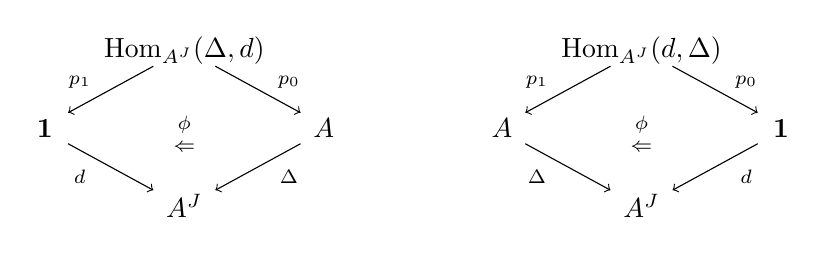
\begin{tikzpicture}[x=1.4em,y=1.4em]
  \node (h) at (0,0) {$\mathrm{Hom}_{A^{J}}(\Delta,d)$};
  \node (one) at (-3.6,-2.0) {$\qcOne$};
  \node (a) at (3.6,-2.0) {$A$};
  \node (aj) at (0,-4.0) {$A^{J}$};
  \draw[->] (-0.8,-0.4) -- (-3.0,-1.6);
  \node at (-2.7,-0.8) {$\scriptstyle p_{1}$};
  \draw[->] (0.8,-0.4) -- (3.0,-1.6);
  \node at (2.7,-0.8) {$\scriptstyle p_{0}$};
  \draw[->] (-3.0,-2.4) -- (-0.8,-3.6);
  \node at (-2.7,-3.25) {$\scriptstyle d$};
  \draw[->] (3.0,-2.4) -- (0.8,-3.6);
  \node at (2.7,-3.25) {$\scriptstyle\Delta$};
  \node at (0,-1.9) {$\scriptstyle\phi$};
  \node at (0,-2.5) {$\scriptstyle\Leftarrow$};
  \begin{scope}[shift={(11.8,0)}]
  \node (h2) at (0,0) {$\mathrm{Hom}_{A^{J}}(d,\Delta)$};
  \node (a2) at (-3.6,-2.0) {$A$};
  \node (one2) at (3.6,-2.0) {$\qcOne$};
  \node (aj2) at (0,-4.0) {$A^{J}$};
  \draw[->] (-0.8,-0.4) -- (-3.0,-1.6);
  \node at (-2.7,-0.8) {$\scriptstyle p_{1}$};
  \draw[->] (0.8,-0.4) -- (3.0,-1.6);
  \node at (2.7,-0.8) {$\scriptstyle p_{0}$};
  \draw[->] (-3.0,-2.4) -- (-0.8,-3.6);
  \node at (-2.7,-3.25) {$\scriptstyle\Delta$};
  \draw[->] (3.0,-2.4) -- (0.8,-3.6);
  \node at (2.7,-3.25) {$\scriptstyle d$};
  \node at (0,-1.9) {$\scriptstyle\phi$};
  \node at (0,-2.5) {$\scriptstyle\Leftarrow$};
  \end{scope}
\end{tikzpicture}
\end{center}

将诸\trCospan{}中「\trDiagram{}」那一支替换掉，\cref{def:infinity-category-of-cones}%
便可修改成容许 $d\colon D\to A^{J}$ 为一族\trDiagram{}的形式。在泛情形
（即 $d$ 为恒同\trFunctor{} $\mathrm{id}_{A^{J}}\colon A^{J}\to A^{J}$ 时）下，%
这就定义了形状 $J$ 的任意\trDiagram{}之上或之下的\trInfinityCategoryOfCones{}%
$\mathrm{Hom}_{A^{J}}(\Delta,A^{J})$。

在索引形状 $J$ 为一个\trSimplicialSet（而非\trCartesianClosed{}\trInfinityCosmos{}%
中的一个\trInfinityCategory）的情形，\trDiagram{}之上或之下的%
\trInfinityCategoryOfCones{}还有另一个模型：它可以由最初由 Ehlers 与 Porter
\cite{bib40} 发展出的单纯\trJoin（join）构造建造出来。
诸模型之间的\trEquivalence{}，是\trJoin{}运算与 Joyal \cite[\S9]{bib63} 引入的
所谓「\trFatJoin」（fat join）之间的\trEquivalence{}的一个推论。
正如\cref{lem:fat-join-cones}所揭示的，\trFatJoin{}构造的一个特殊实例给出%
\cref{def:infinity-category-of-cones}中出现的那些\trCone{}的形状。我们
现在引入这些概念。

\begin{definition}[\trFatJoin]\label{def:fat-join}
单纯集 $I$ 与 $J$ 的\textbf{\trFatJoin}是由如下\trPushout{}构造出的\trSimplicialSet：
\begin{center}
\begin{tikzpicture}[x=1.5em,y=1.5em]
  \node (tl) at (0,1.5) {$(I\times J)\sqcup(I\times J)$};
  \node (tr) at (7.2,1.5) {$I\sqcup J$};
  \node (bl) at (0,-1.5) {$I\times\qcTwo\times J$};
  \node (br) at (7.2,-1.5) {$I\diamond J$};
  \draw[->] (3.3,1.5) -- node[above]{$\scriptstyle\pi_{J}\sqcup\pi_{J}$} (5.5,1.5);
  \draw[right hook->] (0,0.9) -- (0,-0.9);
  \node at (2.0,0) {$\scriptstyle\ulcorner$};
  \draw[->] (2.6,-1.5) -- (5.5,-1.5);
\end{tikzpicture}
\end{center}
由此可得
\begin{equation*}
(I\diamond J)_{n}:=I_{n}\sqcup\Bigl(\coprod_{[n]\to[1]}I_{n}\times J_{n}\Bigr)\sqcup J_{n}.
\end{equation*}
注意存在自然映射 $I\diamond J\twoheadrightarrow\qcTwo$，由投影
$\pi\colon I\times\qcTwo\times J\twoheadrightarrow\qcTwo$ 诱导，使得 $I$ 是
$0$ 之上的纤维、而 $J$ 是 $1$ 之上的纤维：
\begin{center}
\begin{tikzpicture}[x=1.5em,y=1.5em]
  \node (tl) at (0,1.5) {$I\sqcup J$};
  \node (tr) at (4.6,1.5) {$I\diamond J$};
  \node (bl) at (0,-1.5) {$\qcOne+\qcOne$};
  \node (br) at (4.6,-1.5) {$\qcTwo$};
  \draw[right hook->] (1.1,1.5) -- (3.5,1.5);
  \draw[->] (0,0.9) -- (0,-0.9);
  \node at (1.6,0) {$\scriptstyle\lrcorner$};
  \draw[->] (1.3,-1.5) -- node[below]{$\scriptstyle(0,1)$} (3.3,-1.5);
\end{tikzpicture}
\end{center}
\end{definition}

任意形状为 $J$ 的\trDiagram{}之上或之下的\trInfinityCategoryOfCones{}%
可以重新描述如下。

\begin{lemma}\label{lem:fat-join-cones}
对\trInfinityCosmos{} $\mathcal{K}$ 中的任何\trSimplicialSet{} $J$ 与任何%
\trInfinityCategory{} $A$，我们有自然同构
\begin{equation*}
\mathrm{Hom}_{A^{J}}(\Delta,A^{J})\cong A^{\qcOne\diamond J}
\qquad\text{及}\qquad
\mathrm{Hom}_{A^{J}}(A^{J},\Delta)\cong A^{J\diamond\qcOne}.
\end{equation*}
\end{lemma}

\begin{proof}
单纯\trCotensor{} $A^{(-)}\colon\sSet^{\mathrm{op}}\to\mathcal{K}$ 把%
\cref{def:fat-join}的\trPushout{}送到把 $\Delta\colon A\to A^{J}$ 表示为一个%
\trCommaInfinityCategory{}的左表示与右表示所定义的那些拉回方块：
\begin{center}
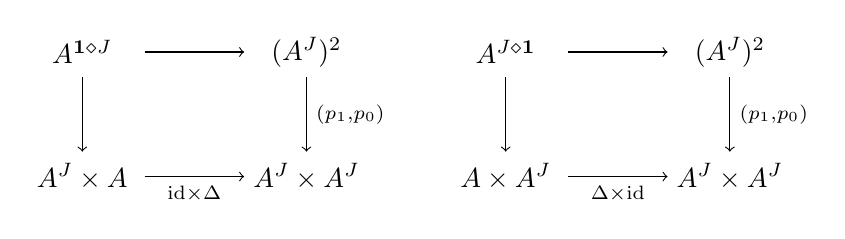
\begin{tikzpicture}[x=1.5em,y=1.5em]
  \node (tl) at (0,1.5) {$A^{\qcOne\diamond J}$};
  \node (tr) at (5.4,1.5) {$(A^{J})^{2}$};
  \node (bl) at (0,-1.5) {$A^{J}\times A$};
  \node (br) at (5.4,-1.5) {$A^{J}\times A^{J}$};
  \draw[->] (1.5,1.5) -- (3.9,1.5);
  \draw[->] (0,0.9) -- (0,-0.9);
  \node at (1.5,0) {$\scriptstyle\lrcorner$};
  \draw[->] (5.4,0.9) -- node[right]{$\scriptstyle(p_{1},p_{0})$} (5.4,-0.9);
  \draw[->] (1.5,-1.5) -- node[below]{$\scriptstyle\mathrm{id}\times\Delta$} (3.9,-1.5);
  \begin{scope}[shift={(10.2,0)}]
  \node (tl2) at (0,1.5) {$A^{J\diamond\qcOne}$};
  \node (tr2) at (5.4,1.5) {$(A^{J})^{2}$};
  \node (bl2) at (0,-1.5) {$A\times A^{J}$};
  \node (br2) at (5.4,-1.5) {$A^{J}\times A^{J}$};
  \draw[->] (1.5,1.5) -- (3.9,1.5);
  \draw[->] (0,0.9) -- (0,-0.9);
  \node at (1.5,0) {$\scriptstyle\lrcorner$};
  \draw[->] (5.4,0.9) -- node[right]{$\scriptstyle(p_{1},p_{0})$} (5.4,-0.9);
  \draw[->] (1.5,-1.5) -- node[below]{$\scriptstyle\Delta\times\mathrm{id}$} (3.9,-1.5);
  \end{scope}
\end{tikzpicture}
\end{center}
\end{proof}

\begin{definition}[\trJoin，D.2.6]\label{def:join}
单纯集 $I$ 与 $J$ 的\textbf{\trJoin}是单纯集 $I\star J$
\begin{center}
\begin{tikzpicture}[x=1.5em,y=1.5em]
  \node (tl) at (0,1.5) {$I\sqcup J$};
  \node (tr) at (4.6,1.5) {$I\star J$};
  \node (bl) at (0,-1.5) {$\qcOne+\qcOne$};
  \node (br) at (4.6,-1.5) {$\qcTwo$};
  \draw[right hook->] (1.1,1.5) -- (3.5,1.5);
  \draw[->] (0,0.9) -- (0,-0.9);
  \node at (1.6,0) {$\scriptstyle\lrcorner$};
  \draw[->] (1.3,-1.5) -- node[below]{$\scriptstyle(0,1)$} (3.3,-1.5);
\end{tikzpicture}
\qquad
其中 $\displaystyle(I\star J)_{n}:=I_{n}\sqcup\Bigl(\coprod_{0\leq k<n}I_{n-k-1}\times J_{k}\Bigr)\sqcup J_{n}$
\end{center}
并且这些 $n$-单纯形的诸顶点带有定向，使得存在典范映射
$I\star J\to\qcTwo$，其中 $I$ 是 $0$ 之上的纤维、而 $J$ 是 $1$ 之上的纤维
（更多细节见定义 D.2.2 与 D.2.6，或原始文献 \cite{bib40} 与
\cite[\S3]{bib61}）。
\end{definition}

\trJoin{}函子 $-\star J\colon\sSet\to\sSet$ 保持连通余极限，但不保持\trInitial{}对象
与其他\trCoproduct；不过，把余定义域换成 $J$ 之下的切片范畴便可达成余连续性：
函子 $-\star J\colon\sSet\to{}^{J/}\!\sSet$ 保持一切余极限（见引理 D.2.7）。
在这一语境化之下，\trJoin{}容许一个\trRightAdjoint，它由 Joyal 的\textbf{切片}%
（slice）构造定义：后者把\trSimplicialMap{} $f\colon J\to X$ 送到传统上记作 $X_{/f}$
的单纯集。

\begin{proposition}[\trJoin$\dashv$切片伴随]\label{prop:join-slice-adjunction}
诸\trJoin{}函子容许由如下自然双射定义的\trRightAdjoint：
\begin{center}
\mbox{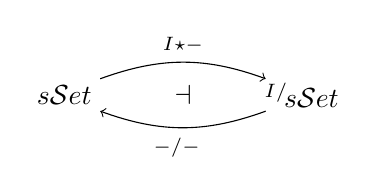
\begin{tikzpicture}[x=1.3em,y=1.3em]
  \node (s) at (0,0) {$\sSet$};
  \node (j) at (6.6,0) {${}^{I/}\!\sSet$};
  \draw[->] (1.0,0.45) to[bend left=20] node[above]{$\scriptstyle I\star-$} (5.6,0.45);
  \node at (3.3,0) {$\dashv$};
  \draw[->] (5.6,-0.45) to[bend left=20] node[below]{$\scriptstyle-/-\;\;{}$} (1.0,-0.45);
\end{tikzpicture}}
\qquad
$\left\{\,\Delta[n]\to{}^{h/}\!\!X\,\right\}:=
\left\{\vcenter{\hbox{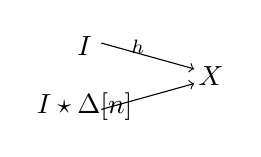
\begin{tikzpicture}[x=1.2em,y=1.2em]
  \node (i) at (0,0.9) {$I$};
  \node (m) at (0,-0.9) {$I\star\Delta[n]$};
  \node (x) at (3.8,0) {$X$};
  \draw[->] (0.5,1.0) -- (3.3,0.22);
  \node at (1.6,0.88) {$\scriptstyle h$};
  \draw[->] (0.5,-1.0) -- (3.3,-0.22);
\end{tikzpicture}}}\right\}$
\end{center}
\begin{center}
\mbox{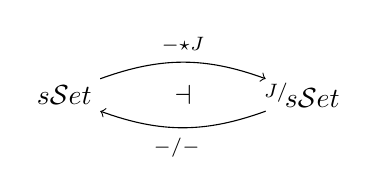
\begin{tikzpicture}[x=1.3em,y=1.3em]
  \node (s) at (0,0) {$\sSet$};
  \node (j) at (6.6,0) {${}^{J/}\!\sSet$};
  \draw[->] (1.0,0.45) to[bend left=20] node[above]{$\scriptstyle-\star J$} (5.6,0.45);
  \node at (3.3,0) {$\dashv$};
  \draw[->] (5.6,-0.45) to[bend left=20] node[below]{$\scriptstyle-/-\;\;{}$} (1.0,-0.45);
\end{tikzpicture}}
\qquad
$\left\{\,\Delta[n]\to X_{/k}\,\right\}:=
\left\{\vcenter{\hbox{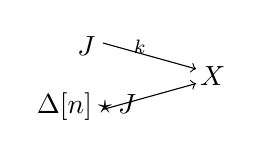
\begin{tikzpicture}[x=1.2em,y=1.2em]
  \node (i) at (0,0.9) {$J$};
  \node (m) at (0,-0.9) {$\Delta[n]\star J$};
  \node (x) at (3.8,0) {$X$};
  \draw[->] (0.5,1.0) -- (3.3,0.22);
  \node at (1.6,0.88) {$\scriptstyle k$};
  \draw[->] (0.5,-1.0) -- (3.3,-0.22);
\end{tikzpicture}}}\right\}$
\end{center}
\end{proposition}

\begin{proof}
单纯集 $X_{/k}$ 定义为其 $n$-单纯形对应于 $J$ 之下的那些映射
$\Delta[n]\star J\to X$，其上的右作用由单纯算子 $[m]\to[n]$ 经
$\Delta[m]\to\Delta[n]$ 的\trPreComposition{}给出。由于\trJoin{}函子
$-\star J\colon\sSet\to{}^{J/}\!\sSet$ 保持余极限，这就扩充成一个介于映射
$I\to X_{/k}$ 与 $J$ 之下的那些映射 $I\star J\to X$ 之间的双射，且该双射在
$I$ 与 $k\colon J\to X$ 中均自然。
\end{proof}

\begin{notation}\label{not:cone-notation}
对任何\trSimplicialSet{} $J$，我们记
\begin{equation*}
J^{\triangleleft}:=\qcOne\star J
\qquad\text{与}\qquad
J^{\triangleright}:=J\star\qcOne
\end{equation*}
并以 $\top$ 记 $J^{\triangleleft}$ 的、由终单纯集 $\qcOne$ 所贡献的那个%
\textbf{\trCone{}顶点}（cone vertex），以 $\bot$ 记 $J^{\triangleright}$ 的%
\trCone{}顶点。这些单纯集配备有典范包含
\begin{equation*}
J^{\triangleleft}\hookleftarrow J\hookrightarrow J^{\triangleright}
\end{equation*}
\end{notation}

正如其名所示，\trJoin{}与\trFatJoin{}这两个构造定义出的索引形状是彼此等价的，其意义如下。

\begin{proposition}[\trJoin{}与\trFatJoin]\label{prop:join-vs-fat-join}
对任何单纯集 $I$ 与 $J$ 以及任何\trInfinityCategory{} $A$，存在自然等价
\begin{center}
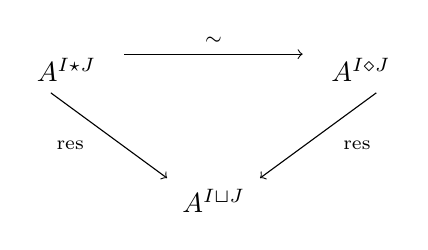
\begin{tikzpicture}[x=1.4em,y=1.4em]
  \node (l) at (0,1.6) {$A^{I\star J}$};
  \node (r) at (7.6,1.6) {$A^{I\diamond J}$};
  \node (b) at (3.8,-1.8) {$A^{I\sqcup J}$};
  \draw[->] (1.5,2.0) -- node[above]{$\scriptstyle\sim$} (6.1,2.0);
  \draw[->] (-0.4,1.0) -- (2.6,-1.2);
  \node at (0.1,-0.35) {$\scriptstyle\mathrm{res}$};
  \draw[->] (8.0,1.0) -- (5.0,-1.2);
  \node at (7.5,-0.35) {$\scriptstyle\mathrm{res}$};
\end{tikzpicture}
\end{center}
\end{proposition}

\begin{proof}
存在单纯集之间的一个典范映射
\begin{center}
\begin{tikzpicture}[x=1.5em,y=1.5em]
  \node (tl) at (0,1.6) {$(I\times J)\sqcup(I\times J)$};
  \node (tr) at (7.6,1.6) {$I\sqcup J$};
  \node (ml) at (0,-1.6) {$I\times\qcTwo\times J$};
  \node (mm) at (5.8,-1.6) {$I\diamond J$};
  \node (mr) at (10.8,-1.6) {$I\star J$};
  \node (bt) at (5.8,-4.6) {$\qcTwo$};
  \draw[->] (3.4,1.6) -- node[above]{$\scriptstyle\pi_{J}\sqcup\pi_{J}$} (5.7,1.6);
  \draw[->] (0,1.0) -- (0,-1.0);
  \node at (2.2,-0.1) {$\scriptstyle\ulcorner$};
  \draw[->] (2.4,-1.6) -- (4.5,-1.6);
  \draw[->,dashed] (7.1,-1.6) -- (9.5,-1.6);
  \draw[->] (8.1,1.3) -- (10.4,-1.1);
  \draw[->] (5.8,-2.2) -- (5.8,-4.0);
  \draw[->] (0.4,-2.2) -- (5.0,-4.4);
  \draw[->] (10.3,-2.1) -- (6.7,-4.3);
\end{tikzpicture}
\end{center}
该映射与诸纤维 $I\sqcup J$ 的包含相交换，并卧于到 $\qcTwo$ 的诸投影之上。
$I\diamond J$ 中一个不居于任一纤维之内的 $n$-单纯形，由如下三元组的数据
给定：$(\alpha\colon[n]\twoheadrightarrow[1],\ \sigma\in I_{n},\ \tau\in J_{n})$。虚线映射把这个单纯形送到代表 $I\star J$ 的一个 $n$-单纯形
的二元组 $(\sigma|_{[0,\dots,k]}\in I_{k},\ \tau|_{[k+1,\dots,n]}\in J_{n-k-1})$，其中 $k\in[n]$ 是 $\alpha^{-1}(0)$ 中的
最大顶点。附录 D 中的\cref{prop:fat-join-comparison-weak-equivalence}，
或 Lurie 的 \cite[4.2.1.2]{bib78}，证明了该映射在
$Q^{I}\times Q^{J}$ 之上诱导出诸\trQuasiCategory{}的自然等价
$Q^{I\star J}\rightsquigarrow Q^{I\diamond J}$。取 $Q$ 为\trFunctorSpace{}
$\mathrm{Fun}(X,A)$，便对一般的∞-\trCategory{}证得所宣称的等价。
\end{proof}

\begin{corollary}\label{cor:comma-squares}
对任何\trSimplicialSet{} $J$ 与\trInfinityCategory{} $A$，存在\trCommaSquare%
（comma squares）
\begin{rveq}\label{eq:comma-squares}
\mbox{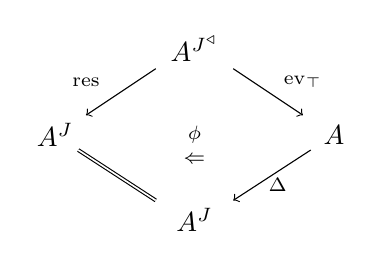
\begin{tikzpicture}[x=1.4em,y=1.4em]
  \node (t) at (0,0) {$A^{J^{\triangleleft}}$};
  \node (l) at (-3.6,-2.2) {$A^{J}$};
  \node (r) at (3.6,-2.2) {$A$};
  \node (b) at (0,-4.4) {$A^{J}$};
  \draw[->] (-1.0,-0.5) -- (-2.8,-1.7);
  \node at (-2.8,-0.85) {$\scriptstyle\mathrm{res}$};
  \draw[->] (1.0,-0.5) -- (2.8,-1.7);
  \node at (2.8,-0.85) {$\scriptstyle\mathrm{ev}_{\top}$};
  \node at (0,-2.2) {$\scriptstyle\phi$};
  \node at (0,-2.85) {$\scriptstyle\Leftarrow$};
  \draw[double] (-3.0,-2.6) -- (-1.0,-3.9);
  \draw[->] (3.0,-2.6) -- (1.0,-3.9);
  \node at (2.15,-3.5) {$\scriptstyle\Delta$};
\end{tikzpicture}}
\qquad
\mbox{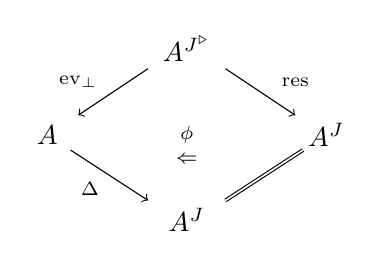
\begin{tikzpicture}[x=1.4em,y=1.4em]
  \node (t) at (0,0) {$A^{J^{\triangleright}}$};
  \node (l) at (-3.6,-2.2) {$A$};
  \node (r) at (3.6,-2.2) {$A^{J}$};
  \node (b) at (0,-4.4) {$A^{J}$};
  \draw[->] (-1.0,-0.5) -- (-2.8,-1.7);
  \node at (-2.8,-0.85) {$\scriptstyle\mathrm{ev}_{\bot}$};
  \draw[->] (1.0,-0.5) -- (2.8,-1.7);
  \node at (2.8,-0.85) {$\scriptstyle\mathrm{res}$};
  \node at (0,-2.2) {$\scriptstyle\phi$};
  \node at (0,-2.85) {$\scriptstyle\Leftarrow$};
  \draw[->] (-3.0,-2.6) -- (-1.0,-3.9);
  \node at (-2.5,-3.6) {$\scriptstyle\Delta$};
  \draw[double] (1.0,-3.9) -- (3.0,-2.6);
\end{tikzpicture}}
\end{rveq}
它们沿一族\trDiagram{} $d\colon D\to A^{J}$ 作拉回，给出 $d$ 之上或之下的%
\trInfinityCategoryOfCones{}的\trEquivalence{}模型：
\begin{center}
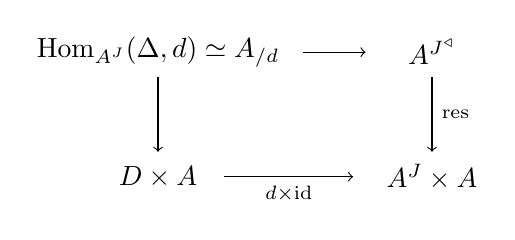
\begin{tikzpicture}[x=1.5em,y=1.5em]
  \node (h) at (0,1.5) {$\mathrm{Hom}_{A^{J}}(\Delta,d)\simeq A_{/d}$};
  \node (aj) at (6.6,1.5) {$A^{J^{\triangleleft}}$};
  \node (da) at (0,-1.5) {$D\times A$};
  \node (aa) at (6.6,-1.5) {$A^{J}\times A$};
  \draw[->] (3.5,1.5) -- (5.0,1.5);
  \draw[->] (0,0.9) -- (0,-0.9);
  \draw[->] (6.6,0.9) -- node[right]{$\scriptstyle\mathrm{res}$} (6.6,-0.9);
  \draw[->] (1.6,-1.5) -- node[below]{$\scriptstyle d\times\mathrm{id}$} (4.7,-1.5);
  \node at (2.5,-0.35) {$\scriptstyle\lrcorner$};
\end{tikzpicture}
\qquad
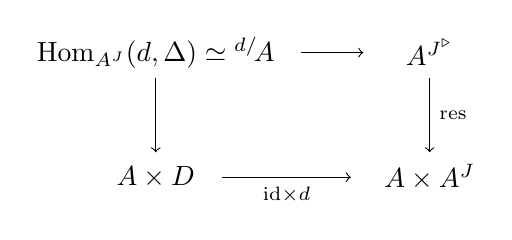
\begin{tikzpicture}[x=1.5em,y=1.5em]
  \node (h) at (0,1.5) {$\mathrm{Hom}_{A^{J}}(d,\Delta)\simeq{}^{d/}\!A$};
  \node (aj) at (6.6,1.5) {$A^{J^{\triangleright}}$};
  \node (da) at (0,-1.5) {$A\times D$};
  \node (aa) at (6.6,-1.5) {$A\times A^{J}$};
  \draw[->] (3.5,1.5) -- (5.0,1.5);
  \draw[->] (0,0.9) -- (0,-0.9);
  \draw[->] (6.6,0.9) -- node[right]{$\scriptstyle\mathrm{res}$} (6.6,-0.9);
  \draw[->] (1.6,-1.5) -- node[below]{$\scriptstyle\mathrm{id}\times d$} (4.7,-1.5);
  \node at (2.5,-0.35) {$\scriptstyle\lrcorner$};
\end{tikzpicture}
\end{center}
\end{corollary}

\begin{proof}
\cref{prop:join-vs-fat-join}构造出纤维化等价
$A^{\qcOne\diamond J}\simeq_{A^{J}\times A}A^{J^{\triangleleft}}$ 与
$A^{J\diamond\qcOne}\simeq_{A\times A^{J}}A^{J^{\triangleright}}$。由%
\cref{lem:fat-join-cones}，$A^{\qcOne\diamond J}$ 与 $A^{J\diamond\qcOne}$
是\trCommaInfinityCategory。于是，命题 3.4.11 蕴含：这些纤维化等价为
$A^{J^{\triangleleft}}$ 与 $A^{J^{\triangleright}}$ 配备上\trCommaCone，满足
命题 3.4.6 的弱\trUniversalProperty。\cref{eq:comma-squares}中的诸%
\trNaturalTransformation{}由如下诸水平复合表示
\begin{center}
\begin{tikzpicture}[x=1.4em,y=1.4em]
  \node (tl) at (0,1.6) {$J\sqcup J$};
  \node (tr) at (5.2,1.6) {$\qcOne\sqcup J$};
  \node (bl) at (0,-1.6) {$J\times\qcTwo$};
  \node (mm) at (5.2,-1.6) {$\qcOne\diamond J$};
  \node (mr) at (9.4,-1.6) {$J^{\triangleleft}$};
  \node (bt) at (5.2,-4.6) {$\qcTwo$};
  \draw[->] (1.5,1.6) -- (3.7,1.6);
  \draw[->] (0,1.0) -- (0,-1.0);
  \node at (1.7,-0.1) {$\scriptstyle\ulcorner$};
  \draw[->] (1.9,-1.6) -- (3.9,-1.6);
  \draw[->,dashed] (6.5,-1.6) -- (8.1,-1.6);
  \draw[->] (5.7,1.3) -- (9.0,-1.1);
  \draw[->] (5.2,-2.2) -- (5.2,-4.0);
  \draw[->] (0.4,-2.2) -- (4.4,-4.4);
  \draw[->] (8.9,-2.1) -- (6.1,-4.3);
\end{tikzpicture}
\qquad
\begin{tikzpicture}[x=1.4em,y=1.4em]
  \node (tl) at (0,1.6) {$J\sqcup J$};
  \node (tr) at (5.2,1.6) {$J\sqcup\qcOne$};
  \node (bl) at (0,-1.6) {$J\times\qcTwo$};
  \node (mm) at (5.2,-1.6) {$J\diamond\qcOne$};
  \node (mr) at (9.4,-1.6) {$J^{\triangleright}$};
  \node (bt) at (5.2,-4.6) {$\qcTwo$};
  \draw[->] (1.5,1.6) -- (3.7,1.6);
  \draw[->] (0,1.0) -- (0,-1.0);
  \node at (1.7,-0.1) {$\scriptstyle\ulcorner$};
  \draw[->] (1.9,-1.6) -- (3.9,-1.6);
  \draw[->,dashed] (6.5,-1.6) -- (8.1,-1.6);
  \draw[->] (5.7,1.3) -- (9.0,-1.1);
  \draw[->] (5.2,-2.2) -- (5.2,-4.0);
  \draw[->] (0.4,-2.2) -- (4.4,-4.4);
  \draw[->] (8.9,-2.1) -- (6.1,-4.3);
\end{tikzpicture}
\end{center}
将它们作\trCotensor{}射入 $A$，便产生自然变换：
\begin{center}
\begin{tikzpicture}[x=1.15em,y=1.4em]
  \node (l) at (0,0) {$A^{J^{\triangleleft}}$};
  \node (m) at (6.0,0) {$(A^{J})^{2}$};
  \node (r) at (12.0,0) {$A^{J}$};
  \draw[->] (1.9,0.35) to[bend left=18] (4.7,0.35);
  \node at (3.0,1.05) {$\scriptstyle\Delta\mathrm{ev}_{\top}$};
  \draw[->] (1.9,-0.35) to[bend right=18] (4.7,-0.35);
  \node at (3.0,-1.05) {$\scriptstyle\mathrm{res}$};
  \draw[->] (7.4,0.35) to[bend left=18] (10.5,0.35);
  \node at (8.4,1.05) {$\scriptstyle p_{0}$};
  \draw[->] (8.95,0.2) to[bend right=35] (8.95,-0.2);
  \node at (9.95,0) {$\scriptstyle\psi_{\kappa}$};
  \node at (8.4,-1.05) {$\scriptstyle p_{1}$};
  \draw[->] (7.4,-0.35) to[bend right=18] (10.5,-0.35);
  \node at (14.6,0) {与};
  \begin{scope}[shift={(17.2,0)}]
  \node (l2) at (0,0) {$A^{J^{\triangleright}}$};
  \node (m2) at (6.0,0) {$(A^{J})^{2}$};
  \node (r2) at (12.0,0) {$A^{J}$};
  \draw[->] (1.9,0.35) to[bend left=18] (4.7,0.35);
  \node at (3.0,1.05) {$\scriptstyle\mathrm{res}$};
  \draw[->] (1.9,-0.35) to[bend right=18] (4.7,-0.35);
  \node at (3.0,-1.05) {$\scriptstyle\Delta\mathrm{ev}_{\bot}$};
  \draw[->] (7.4,0.35) to[bend left=18] (10.5,0.35);
  \node at (8.4,1.05) {$\scriptstyle p_{0}$};
  \draw[->] (8.95,0.2) to[bend right=35] (8.95,-0.2);
  \node at (9.95,0) {$\scriptstyle\psi_{\kappa}$};
  \node at (8.4,-1.05) {$\scriptstyle p_{1}$};
  \draw[->] (7.4,-0.35) to[bend right=18] (10.5,-0.35);
  \end{scope}
\end{tikzpicture}
\end{center}
这些纤维化等价经拉回，即为固定的一族\trDiagram{} $d$ 之上或之下的%
\trInfinityCategoryOfCones{}给出\trEquivalence{}的模型。
\end{proof}

\begin{warning}\label{war:slice-notation}
在\cref{cor:comma-squares}的陈述与其他场合，对\trDiagram{}
$d\colon\qcOne\to A^{J}$ 之上的诸限制映射的诸\trFiber，借用 Joyal 的切片
记号颇为便利。这一用法的正当性由附录 D 中的%
\cref{prop:slices-cones-equivalence}给出：后者在\trQuasiCategory{}%
的\trInfinityCosmos{}中证明 $A_{/d}\simeq_{A}\mathrm{Hom}_{A^{J}}(\Delta,d)$
与 ${}^{d/}\!A\simeq_{A}\mathrm{Hom}_{A^{J}}(d,\Delta)$。然而请注意，在%
\trQuasiCategory{}的\trInfinityCosmos{}中，这些严格纤维并\emph{不}同构于
Joyal 的切片拟范畴（见\cref{ex:fiber-of-cone-category}），而仅仅是等价于
它们。
\end{warning}

\subsection*{练习}

\begin{exercise}\label{ex:join-vs-fat-join-section}
计算 $\Delta[n]\star\Delta[m]$ 与 $\Delta[n]\diamond\Delta[m]$，并对%
\cref{prop:join-vs-fat-join}之证明中所构造的那个映射定义一个\trSection
\begin{equation*}
\Delta[n]\star\Delta[m]\longrightarrow\Delta[n]\diamond\Delta[m]
\end{equation*}
\end{exercise}

\begin{exercise}\label{ex:fiber-of-cone-category}
在\trQuasiCategory{}的\trInfinityCosmos{}中，计算 $A^{J^{\triangleleft}}\twoheadrightarrow A^{J}$ 在 $d\colon\qcOne\to A^{J}$ 之上的\trFiber，并
证明该\trQuasiCategory{}不同构于 $A_{/d}$。
\end{exercise}

\begin{exercise}[{\cite[3.5]{bib63}}]\label{ex:join-dependent-product}
作为预层\trCategory{}的单纯集\trCategory{}是\textbf{局部\trCartesianClosed}%
（locally cartesian closed），意思是与任何映射 $f\colon U\to V$ 相关联的%
\trPullback{}函子都容许一个\trRightAdjoint{} $\Pi_{f}$，称为\textbf{依依赖积}%
（dependent product）或\textbf{前推}（pushforward）：
\begin{center}
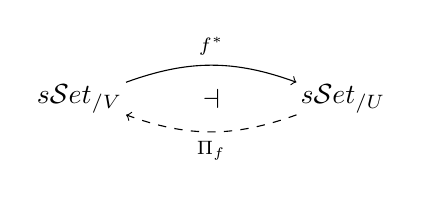
\begin{tikzpicture}[x=1.4em,y=1.4em]
  \node (l) at (0,0) {$\sSet_{/V}$};
  \node (r) at (6.8,0) {$\sSet_{/U}$};
  \draw[->] (1.2,0.42) to[bend left=20] node[above]{$\scriptstyle f^{*}$} (5.6,0.42);
  \node at (3.4,0) {$\dashv$};
  \draw[->,dashed] (5.6,-0.42) to[bend left=20] node[below]{$\scriptstyle\Pi_{f}$} (1.2,-0.42);
\end{tikzpicture}
\end{center}
证明：\trJoin{} $I\star J$ 可以定义为 $\sSet_{/\qcTwo}$ 中的一个对象，即沿
$\qcOne+\qcOne\hookrightarrow\qcTwo$ 取 $!\sqcup!\colon I\sqcup J\to\qcOne+\qcOne$ 的依依赖积。
\end{exercise}
